\documentclass[onecolumn, draftclsnofoot,10pt, compsoc]{IEEEtran}
\usepackage{graphicx}
\usepackage{url}
\usepackage{setspace}
\usepackage[style=numeric,sorting=nty]{biblatex}

\addbibresource{mybib.bib}

%\title{Technology Review: Mixed Reality For Infrastructure Maintenance}
%\author{Team 20: Christopher C Cooper}
%\date{November 2018}

\usepackage{geometry}
\geometry{textheight=9.5in, textwidth=7in}

% 1. Fill in these details
\def \CapstoneTeamName{		xRLucid}
\def \CapstoneTeamNumber{		20}
\def \GroupMemberOne{			Christopher Cooper}
\def \GroupMemberTwo{			Austin Liang}
\def \GroupMemberThree{			David Okubo}
\def \GroupMemberFour{			Jonathan Chen}
\def \GroupMemberFive{			Mingyu Zhang}
\def \CapstoneProjectName{		Mixed Reality for Infrastructure Maintenance}
\def \CapstoneSponsorCompany{	OSU School of Civil and Construction Engineering}
\def \CapstoneSponsorPerson{		Yelda Turkan}

% 2. Uncomment the appropriate line below so that the document type works
\def \DocType{	%	Problem Statement
				%Requirements Document
				%Technology Review
				Design Document
				%Progress Report
				}
			
\newcommand{\NameSigPair}[1]{\par
\makebox[2.75in][r]{#1} \hfil 	\makebox[3.25in]{\makebox[2.25in]{\hrulefill} \hfill		\makebox[.75in]{\hrulefill}}
\par\vspace{-12pt} \textit{\tiny\noindent
\makebox[2.75in]{} \hfil		\makebox[3.25in]{\makebox[2.25in][r]{Signature} \hfill	\makebox[.75in][r]{Date}}}}
% 3. If the document is not to be signed, uncomment the RENEWcommand below
\renewcommand{\NameSigPair}[1]{#1}

%%%%%%%%%%%%%%%%%%%%%%%%%%%%%%%%%%%%%%%
\begin{document}
\begin{titlepage}
    \pagenumbering{gobble}
    \begin{singlespace}
    	\includegraphics[height=4cm]{coe_v_spot1}
        \hfill 
        % 4. If you have a logo, use this includegraphics command to put it on the coversheet.
        %\includegraphics[height=4cm]{CompanyLogo}   
        \par\vspace{.2in}
        \centering
        \scshape{
            \huge CS Capstone \DocType \par
            {\large November 26, 2018}\par
            \vspace{.5in}
            \textbf{\Huge\CapstoneProjectName}\par
            \vfill
            {\large Prepared for}\par
            \Huge \CapstoneSponsorCompany\par
            \vspace{5pt}
            {\Large\NameSigPair{\CapstoneSponsorPerson}\par}
            {\large Prepared by }\par
            Group\CapstoneTeamNumber\par
            % 5. comment out the line below this one if you do not wish to name your team
            \CapstoneTeamName\par 
            \vspace{5pt}
            {\Large
                \NameSigPair{\GroupMemberOne}\par
                \NameSigPair{\GroupMemberTwo}\par
                \NameSigPair{\GroupMemberThree}\par
                \NameSigPair{\GroupMemberFour}\par
                \NameSigPair{\GroupMemberFive}\par
            }
            \vspace{20pt}
        }

\begin{abstract}
This document describes the implementation of the MR for Infrastructure Maintenance system.
The system as proposed is intended to create visualization of BIM information and CAD models for individuals in design, maintenance, and education of Civil and Construction Engineering.
The system has three use cases for a single actor, the user, and seven components.
These components are the 3D model, detailed model information, anchors, internet connection, controls, viewing port.
\end{abstract}
\end{singlespace}
\end{titlepage}
\newpage

%create change history log
%\centering

\pagenumbering{arabic}
\tableofcontents
\listoffigures
%\listoftables
\clearpage

\textbf{Change History}\par

\begin{tabular}{ p{2cm} p{2cm} p{2cm} p{0.25\textwidth} p{0.25\textwidth} }
 \textbf{Revision} & \textbf{Date} & \textbf{Section} & \textbf{Original} & \textbf{New} \\
 \hline
 1.0 & 11/27/2018 & & & Creation of document first draft \\
 \hline
 1.1 & 03/31/2019 & Logical View & New section added. & Removal of BIMData Class and UIPanel Class, noted addition of Button, ScrollList, and Directory classes for each of the UI tasks: browsing the file system, browsing BIM360 hubs, browsing BIM360 issues, browsing BIM360 projects, and browsing BIM360 project files. \\
 \hline
 1.1 & 03/31/2019 & Design Rationale & New section added. & Described need for the new classes due to the inherit nature of Unity 3D
\end{tabular}

\clearpage

\section{Purpose}
The purpose of this document is to describe the proposed implementation of the MR for Infrastructure Maintenance system.
The MR for Infrastructure Maintenance system is designed to provide a mixed reality interface for viewing BIM models for the purpose of construction and maintenance.
\par

\section{Scope}
This document describes the details of implementation of the MR for Infrastructure Maintenance system.
The software will consist of three major functions.
The first function is to render a BIM model, second is to display detailed data from the BIM, and third is adding detailed data to the BIM.
The document will not specify specific BIM data or models.\par

\section{Context}
Maintenance and education in civil and construction engineering has recently started use of BIM with CAD models for maintaining large projects.
These models provide opportunity to create augmented/mixed reality applications to aid those in these fields with the visualization of the designs.
This design document details the method proposed to implement a software system for this visualization.
\par

\section{Summary}
This document provides an overview of the system and its architecture and system design.
In the end, a rationale is presented for the system design.

\section{References}
\newpage
\section{Glossary}

\begin{tabular}{ p{0.1\textwidth} p{0.85\textwidth} }
 BIM & Building Information Model, a model for construction and infrastructure engineering that contains all information about a project from design to demolition. \\
 MR & Mixed Reality, used to reference a software experience where computer graphics and the physical environment are both present in varying degrees.
\end{tabular}

\newpage

\section{Identified Stakeholders}
The stakeholders for this system are the client, Yelda Turkan, the students of Oregon State University School of Civil and Construction Engineering, and the development team.\par

% not all viewpoints are necessary, comment out any that are not needed
% viewpoint sections are meant for defining the name, design concerns, and design language of the viewpoint
% view sections are meant for describing the design view itself
% these don't need to be the sections. This is just for starting point
%\section{Context Viewpoint}
\section{Context View}
The system consists of one actor, the user of the system, and three services.
The primary service of the system is to render a BIM model in a mixed reality environment.
This service is provided to one user of the system that will be viewing the model.
A user may view multiple different models at a single time due to a single BIM file may have multiple modeled components.
This service is extended by viewing more detailed data of the BIM model.
This detailed data may include building material and metric information of the component.
The detailed data view is extended further by adding/editing this detailed data.
These services are modeled in Figure 1 below.
\par
\begin{figure}[ht]
    \centering
    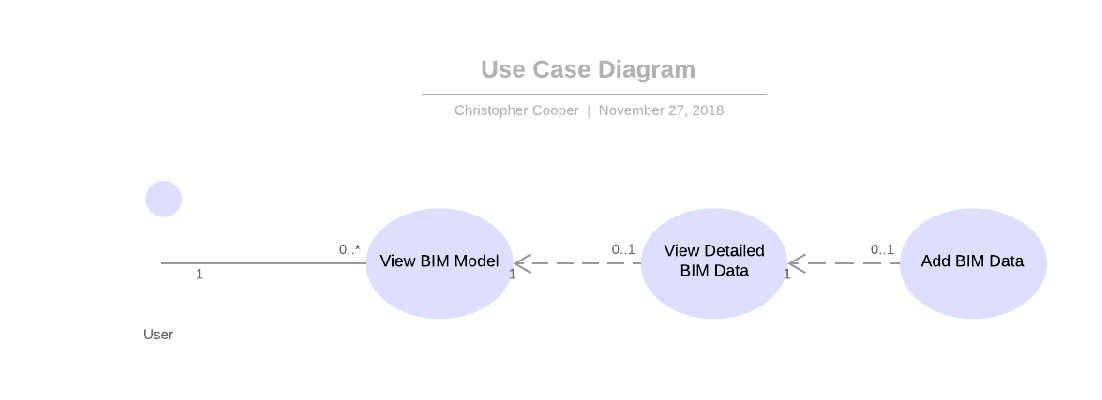
\includegraphics[width=\textwidth]{UseCaseDiag.eps}
    \caption{UML Use Case Diagram}
    \label{fig:UseCaseDiagram}
\end{figure}
The two services extending the rendering of a BIM model component have a maximum of one multiplicity as there is only one set of data to be pulled for each component.
However, both of these services require that the first service is active.
In other words, a model must be loaded and rendered in order to view detailed data.
For the service of adding BIM data, the user will provide input in the form of strings and floats.
The output of the system is a graphics render on a screen of camera feed from the device and the 3D model, as well as display text of detailed data.
\par
\section{Composition View}
The system will have multiple important components to allow for the User to interact with the structure information and allow for the device to communicate with online databases. These include a 3D model visualization, detailed information about the 3D model, Anchors, internet connections, database connections, various user controls, and a viewing port.
\begin{itemize}
    \item \textbf{Overview Model:} 3D model placed in the real world with detailed views of specific structure parts physical model of a structure based on a connected BIM360 database. The overall model will be viewed from afar but also parts of the model can be 'zoomed in' on to show a detailed view.
    \item \textbf{Detailed Model Information:} When viewing the 3D model in a more detailed view (e.g.: viewing a specific structural pillar), BIM360 information will be shown for that portion.
    \item \textbf{Anchors:} The anchors are spots to 'attach' the 3D model to the real world.
    \item \textbf{Internet Connection:} Required to download and upload BIM files.
    \item \textbf{Database Connection:} Connect to a BIM360 database that is related to specific structure.
    \item \textbf{User Controls:} Allows the user to place anchors, move the camera, and interact with model view to change from a overview and a detailed view.
    \item \textbf{Viewing port:} User's 'view point' where the 3D model anchored in the real world can be seen and interacted with. Would zoom into a selected part for a detail view.
\end{itemize}
%\section{Logical Viewpoint}
\section{Logical View}
There are three identified classes for the system shown in Figure 2.
The BIMData class (removed in update 1.1) is a composition of the Model class as the system creates a BIMData object for the Model object, if the user chooses to view detailed data.
The UIPanel class (removed in update 1.1) is an object for creating a window in the Unity Engine to display the BIM data.
The class will get data from the BIMData class using the get\_qualities and get\_quantities methods.\par
\begin{figure}[ht]
    \centering
    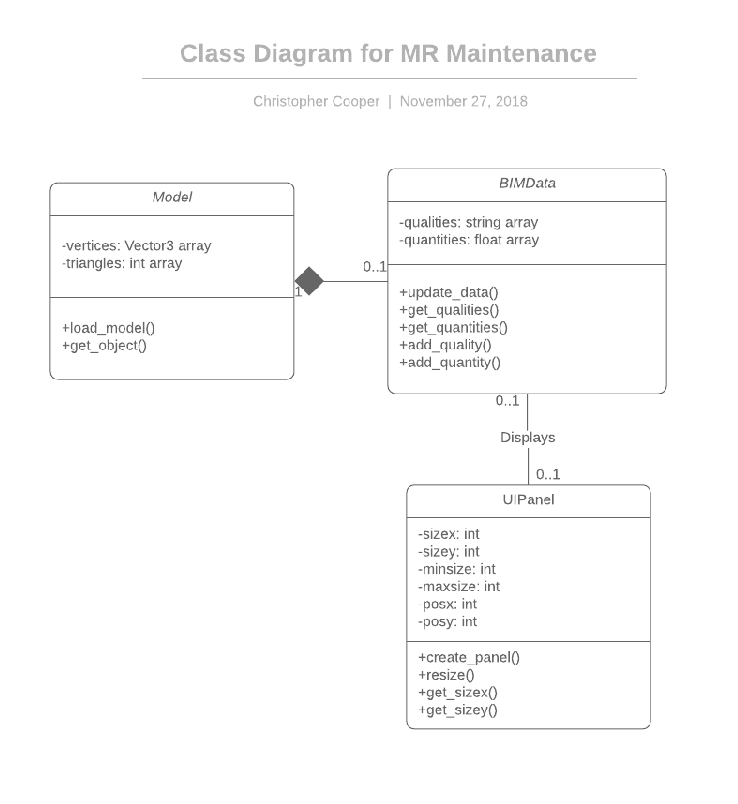
\includegraphics[width=0.5\textwidth]{ClassDiagram.eps}
    \caption{UML Class Diagram}
    \label{fig:ClassDiagram}
\end{figure}
For the use case of adding detailed data, the BIMData class has two additional methods called add\_quantity() and add\_quality() to add new entries into the data of the model.\par

\subsection{Logical View: Update 1.1}
The BIMData class has been removed from the design as the data we receive from the BIM360 API is in the form of a file to be downloaded and opened.
The initial file types to be supported for meta-data are JPEG, PNG, and PDF.
The UIPanel class has also been removed as the only UI required is to find the file the user wants to download.\par
The newly identified classes are the Button, ScrollList, and Directory classes for each UI task.
These UI tasks are browsing the file system, browsing BIM360 hubs, browsing BIM360 issues, browsing BIM360 projects, and browsing BIM360 project files.
Each of these tasks requires unique prefabricated UI components in Unity 3D, thus a unique BUtton, ScrollList, and Directory class will be created for each, utilizing the corresponding prefab components.\par
The ScrollList class is in charge of gathering data needed for the UI either from a BIM360 API call or the system, and populating the UI with buttons for each element of the data gathered.
The common methods of the ScrollList classes are RefreshDisplay(), AddButtons(), and RemoveButtons().
The classes then include supporting methods for retrieving the data to be displayed.
The ScrollList class requires the use of a unique class for each data type needed by the UI including: Hub, Issues, File, Project, and ProjectFile.
The Hub, Issues, Project, and ProjectFile classes are structured as nested classes for automated JSON parsing of the API response.
The Hub class contains the name of the hub from BIM360 and it's ID for accessing BIM360 hubs.
The Issues class contains the strings for created\_at, created\_by, title, and description.
The File class contains the name of the system directory/file, the type of file it is (directory or class), and the icon for it's button.
The Project class contains the id of the project, the name of the project, and the id of the root folder.
Finally the ProjectFile class contains the file ID, displayName, createTime, createUserID, and createUserName.
These relate to the creation of the file in question.\par
The Directory class handles the creation and deletion of the GameObjects in Unity 3d associated with the prefabricated button created for the UI.
This class contains the prefab variable which holds reference to the prefabricated entity the class is supposed to create and a stack of the GameObjects.
The class contains methods GetObject() and ReturnObject().\par
Finally there is the Button class for each UI task.
In general the button contains a reference to the button object in Unity, the ScrollList object it came from, and the class object the button represents.
The Button also includes Unity objects such as Text for any display component of the button.
The methods of the Button classes are Setup() and onCLick().\par

%\section{Dependency View}
%\section{Patterns View}
\section{Interface View}
The system's interface will feature two types of viewing screens and a login screen. The login screen will allow the user to connect the necessary BIM360 database and choose what structure they want to use. The two types of viewing screens will be the 'Model view' and 'Detailed View'.
\begin{itemize}
    \item \textbf{'Model View':} While not in a detailed view of specific part, view port shows simplified 3D model of area of structure in field of view of device's camera
    \item \textbf{'Detailed View':} User can choose a specific part of the model and view more details from the database.  This view zooms in on the specific part of the model.
    \item \textbf{BIM details Menu:} A pop-up menu with BIM information pulled from the BIM360 object.
    \item \textbf{Anchor points:} Pre-determined anchor points visible in the Model View that will be used to allow the user to 'attach' models to keep them in place when moving the device.
    \item \textbf{BIM360 login:} A login menu will be provided to connect to BIM360 database, it will be required before loading anything or accessing the rest of the software. There will be an option for the software to remember the user's login information or staying logged in.
\end{itemize}
\section{Structure View}
A 3D model of the structure from the BIM360 file is displayed on the device's screen, and is anchored in the real-world. The 3D model stays anchored in one location, and allows the user to view different parts of the structure by physically changing the perspective. The user is also able to interact with specific components of the model.

\section{Interaction View}
3D model + Detailed BIM - show BIM for specific part of structure when part is being viewed in a 'detailed' view.

BIM360 + 3D model - 3D model pulled down from BIM360 database

\vspace{1cm}
\textbf{User Input Management}
User input is the information entered by users during the running of the MR application and it is about whole or a piece of the 3d model they are working on, the information could include text, chart, graph, audio, video and more if needed. When such information entered, it should temporarily stay on the running device’s memory since it is time-consuming to go back and forth between hard drive and memory, and then be saved to the hardware and cloud storage when the application is finished. Also, since such information is not entered at once, it needs to keep track of its history to re-display to user properly, and it should be organized in certain format and structure to correctly embed into the interface.\par
The user input management should be part of the main program that displays the 3d model and interacts with the database and local object file. In the main program, the part is unseen until the user required and should be handled as an event during the main loop of the program. When the function is invoked, the program should allow users to enter new information in the interface and allow them to upload image or video as a link or an address of the file. If the entered file is in small size, it should keep in the memory until the program is finished, otherwise saved in hard drive, also for the large size of data like video, it should be entered as a link. When the whole program is finished, it should sort all its original data and the new entered one and write into a file and stored at the hard drive and cloud server, and this part should involve version control system like the database BIM 360 used in the project.\par
The user input management should be implemented at the late stage of the implementation and after when displaying and interaction with the 3d model is finished. The user input management part dependents on the 3d model where the information is attached on, but it could develop separately with the 3d model display when the basic structure is finished. And the test of it should be done by extracting previously entered data and seeing if current entered data is re-displayed properly.


\section{Algorithm View}
World Anchors - the software needs to be able to recognize when the camera is moving, while also keeping the object in place by recognizing anchor points that were placed. The object will be rotated with the device's camera movement to allow the user to view different sides as if it were physically sitting in the real-world.

\section{Resources View}
BIM360 Interfacing - Overall interfacing from BIM360 will be used as a resource for displaying options to users.
%\section{Resources View}

\section{Design Rationale}
The three classes were designed to create the object oriented nature necessary, as a single BIM project may have multiple models, each with their own detailed data for viewing and adding to. There was consideration for an additional class for the anchors that hold the location of the 3D model, however this was changed due to the discovery of the Vuforia SDK plugin for unity. This plugin makes the anchors something the system will interface with, as opposed to creating. The user interface's purpose will be to streamline the start-up process and make interaction and overall use of the software easier to understand and learn. 

The user input management is the part that stores and displays information beside the 3d model and each of the data should link to specific part of the 3d model. Also, the display of such data should be made when rendering the 3d model and in a 3d like structure.\par

\subsection{Design Rationale: Update 1.1}
The creation of the new classes were from Unity needing classes to create each UI object at run time, and dynamically create UI elements on the UI panel.
This meant each button needed to be a class with the Directory classes needed by Unity to generate GameObjects for the Button class to be attached to.
This is largely from the inherit structure of Unity 3D.\par
\end{document}
